\documentclass{article}
\usepackage[utf8]{inputenc}
\usepackage{graphicx}

\title{Sensory Perception}
\author{MCB C61 with Professor David Presti \\ \\ Benjamin Lee}
\date{6 March 2018}

\begin{document}

\maketitle

\textbf{Key Concepts:}
\begin{itemize}
    \item sensation, perception
    \item bacterial chemotaxis
    \item \textit{E. coli} chemotaxis: runs and tumbles
    \item phototropism, phototaxis
    \item naive realism 
    \item electromagnetic spectrum
    \item visible light, ultraviolet, infrared
    \item Karl von Frisch, honeybee vision
    \item pit vipers and infrared
    \item light polarization
    \item audition: very low and very high frequency sound detection
    \item electroreception in sharks
    \item magnetic field sensitivity and animal navigation
\end{itemize}
\newpage

\section{Sensation, Perception}
Sensation of other organisms. We do not know what the sensation or perception of other organisms. What we do know is that we are conscious, but we don't really know how other animals, plants, etc. perceive completely. \\
The brain receives signal information from the environs of the body and uses that information to form mental experiences of the world. This is known as \textit{sensory perception} and is an important nexus between brain, mind and behavior. \\
\textbf{Sensory Perception:} \\
Divided into two basic components:
\begin{enumerate}
    \item \textbf{Sensation:} The collection of information from the environment via sensory organs and receptors
    \item \textbf{Perception:} The analysis and interpretation of this information by the nervous system, contribution to the experience of mental states of perceptual awareness
\end{enumerate}

\section{Bacterial Chemotaxis}
Simple organisms have sensations as well. How do they respond to to the presence of chemical and physical substances? \\

\noindent \textbf{Chemotaxis:} (\textit{chemo}, chemical and \textit{taxis} movement in response to) movement of a motile cell or organism, or part of one, in a direction corresponding to a gradient of increasing or decreasing concentration of a particular substance \\

\noindent They do this via a series of maneuvers called \textbf{Runs and Tumbles}. \\
A \textbf{run} is when a bacteria cell swims in a straight line for a second or so, and then stops swimming and flops for a moment a \textbf{tumble}, it then goes on another run. \\ 
Runs occur when the bacteriums flagella rotate in one direction and bundle to form an effective propeller/motor. Tumbles occur when the direction of flagellar rotation reverses, the flagella fly apart, and motion stops. \\
Mathematically termed as a \textbf{Random Walk} in three dimensions \\

\subsection{\textit{E. coli}}
\begin{itemize}
    \item \textit{Escherichi coli}
    \item 2 micrometers(mm) in length
    \item swims at 30 mm per second, tumbling off in a new direction about every seconds
\end{itemize}
When a bacterium encounters a nutrient chemical substance they respond in a process called \textit{chemotaxis}. Amino acids such as \textit{aspartic acic} and \textit{serine} interact with receptor proteins located on the bacterial cell's outer membrane, causing it to swim toward the chemical. \\

\subsection{Moving Toward Light!}
Light is a prominant environmental stimulus that can influence the behavior of microorganisms, as well as plants and animals. \\

\noindent \textbf{Phototaxis:} process of \textit{entire organism moving} towards light\\
\textbf{Phototropism:} process of \textit{bending or growing} towards light \\

\noindent Organisms that use light as a source (photosynthesis), phototropism and phototaxis helps increase exposure to light. Other organisms that do not derive energy from light, phototropism and phototaxis may enable movement toward a more open region in order to disperse spores or seeds. \\

\noindent \textit{Phycomyces} is a fungus that does not use photosynthesis, but nontheless is extremely sensitive to light. It uses it as a cue to direct the growth of its fruiting bodies called sporangiphores. Uses phototropism to grow in the direction of light. \\

\noindent What do these reactions from \textit{E. coli} and \textit{Phycomyces} say about the mental experiences of perception of these organisms? \\

\section{Naive Realism}
From this discussion we go into how we know what we perceive? In philosphy, there are these two studies that talk about this. \\

\noindent \textit{Ontology}: the study of the nature of reality, what is it that exists? \\
\noindent \textit{Epistemology}: how do we know what we know? \\

According too the conventional framework in the neuroscience of perception, our experience of the world is a function of what actually exists, the physics of our sensory receptors and organs, and the neural manipulation of incoming signals by the brain. \\

However there is this notion in epistemology called \textbf{naive realism}. \\

\noindent \textbf{Naive Realism:} the idea that what we perceive is identical to what actually exists in the world. What we see, hear, smell, taste, and so forth, is exactly what is "out there" in some way. \\
However, the limitations of this notion were clear. Examples such as optical illusions showed that what we see isn't very representative of reality at some points. \\

\section{Electromagnetic Spectrum}
Human sensory perception is sophisticated and limited, there are many physical phenomena that are known to exist, but we are unable to detect naturally. This can be illustrated by taking a look at vision! \\

%https://www.sharelatex.com/learn/Including_images_in_ShareLaTeX
%how to include images in latex
\begin{figure}[htp]
\centering
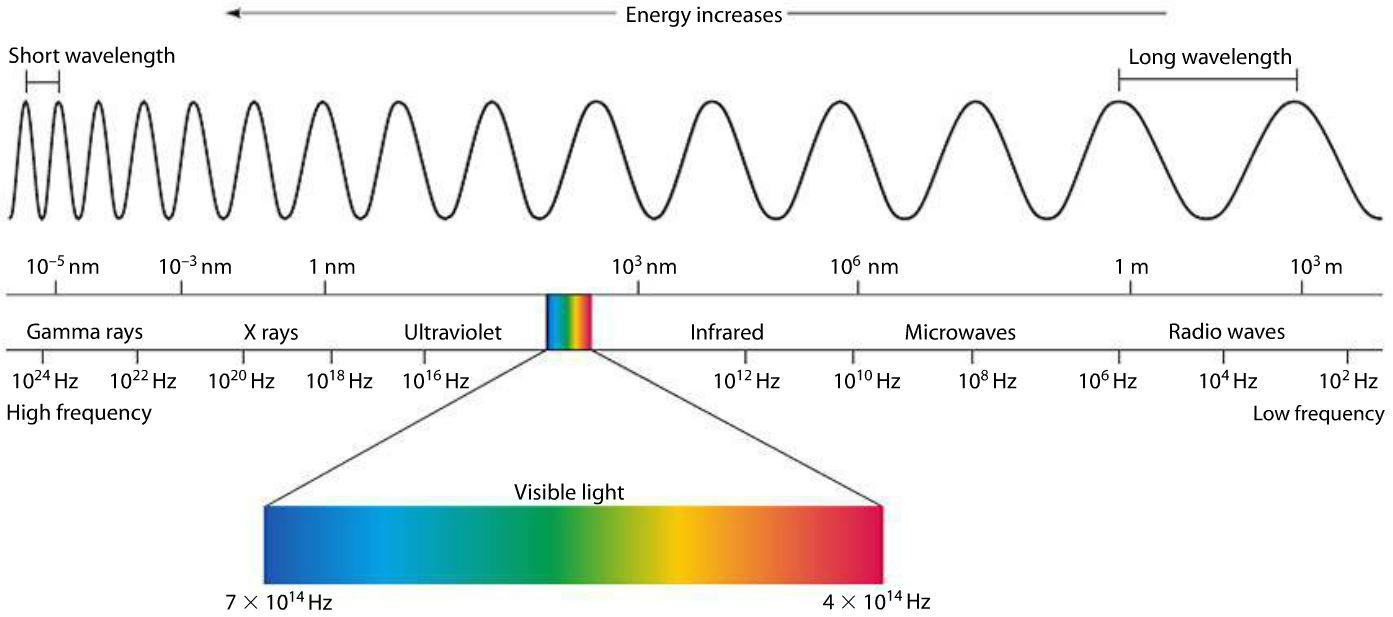
\includegraphics[width=14cm]{images/electro.jpg}
\caption{Electromagnetic Spectrum}
\label{fig:Electromagnetic Spectrum}
\end{figure}

The visual pathway in humans responds to a limited range within the electromagnetic energy spectrum, specifically \textit{visible light}, called this because it is the only part we can see. Spectrum goes from high energy to low energy starting with \\
Gamma rays (high energy) $\rightarrow$ X-ray $\rightarrow$ Ultraviolet $\rightarrow$ Visible Light $\rightarrow$ Infrared $\rightarrow$ Microwave $\rightarrow$ Radio waves (low energy) \\
Gamma and Radio differ by 10$^18$ or a quintillion in energy. \\
Visible Light range \textbf{400nm to 700nm} (high energy, decreasing wavelength $\rightarrow$ low energy, increasing wavelength)\\
\textbf{Ultraviolet} and \textbf{Infrared} are the closest electromagnetic energies to visible light and are seen in nature. \\

\subsection{Ultraviolet Light and Honeybees}
\begin{itemize}
    \item \textbf{Karl von Frisch (1886-1982)} demonstrated that honeybees see color (largely unbelieved at the time)
    \item Won the Nobel Prize for Physiology or Medicine in 1973 (together with Konrad Lorenz and Nikolaas Tinbergen, for work on animal behaviour)
    \item Honeybee visual sensitivity extends into the ultraviolet region of the electromagnetic spectrum. (which humans are blind too)
    \item Discovered these patterns (sometimes called nectar guides) by taking a photo of a flower (specifically shown \textit{Dimorphotheca aurantiaca}) under ultraviolet light. (used as a visual feature to attract bees insects and birds to pollinate them)
\end{itemize}

\begin{figure}[htp]
\centering
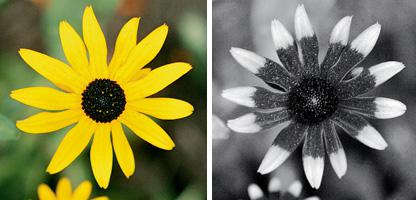
\includegraphics[width=5cm]{images/uvlightflowers.jpg}
\caption{Visible light vs Ultraviolet light}
\label{fig: UV flowers}
\end{figure}

\subsection{Infrared Radiation}

 Another region of the electromagnetic spectrum not visible to humans (energy to low to activate photoreceptors). Absorbed by molecules in such a way as to set them vibrating. Molecular vibratory motion may be experienced as heat. \\
 
 \textbf{Pit Vipers} have the ability to detect infrared radiation using these structures called \textit{pit organs}. They are positioned below the eyes near the nostrils and enable the snake to accurately locate prey animals in darkness. \\

\noindent Two Gadgets that help humans see in the dark: 
\begin{enumerate}
    \item Image intensifier (night vision): amplifies very low intensities of visible light 
    \item Infrared or thermal imager: detects infrared radiation and converts the infrared image to signals in the visible region of the spectrum, allowing things emitting infrared radiation to be seen. 
\end{enumerate}

\subsection{Polarization}
Property of the electromagnetic radiation that can be thought of as the vibration of the electromagnetic field aligned along specific angles in relation to the direction of propagation. \\

\begin{figure}[htp]
\centering
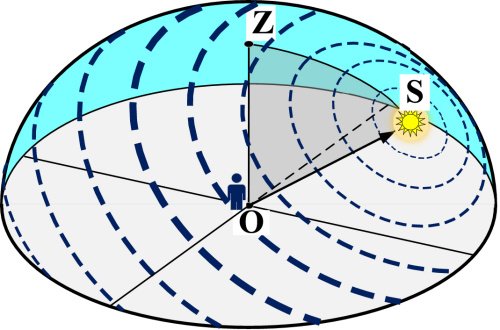
\includegraphics[width=5cm]{images/polarization.jpg}
\caption{Polarization of sunlight across the sky}
\label{fig: Sun Polarization}
\end{figure}

The light from the sun vibrates in all possible angles of polarization, but when reacting with molecules in Earth's atmosphere, it scatters and generates a variation in polarization across the vault of the sky. Meaning the extent to which the light is polarized varies depending on where you look in the sky relative to the sun. \\

The human visual system, without the aid of a polarizing filter, is not sensitive to this property of light. However, insects, reptiles, birds and many other animals are. \\

This discovery was also made by \textbf{Karl von Frisch} in his experiments with honeybees. Using polarizing filters, he was able to conclusively demonstrate that honeybees use sunlight polarization patterns as a navigational aid. Another extraordinary discovery about how animals can see and feel things we can't! \\

\section{Audition: Sound Perception}
Human auditory system is just as sensitive and sophisticated, as with vision, but that means it is also limited. \\

Humans are capable of hearing within \textbf{20 to 20,000 hertz} (Hz) or cycles of vibration per second. Named after Heinrich Hertz (1857 - 1894), a physicist who made contributions to the study of vibrating electromagnetic fields \\

\noindent \textbf{Infrasound:} very \textbf{low-frequency} sound with frequencies \textbf{less than 20 Hz}.
(e.g. Elephants can both generate and hear infrasonic freq and use infrasonic calls while communicating.)\\

\noindent \textbf{Ultrasound:} very \textbf{high-frequency} sound with frequencies \textbf{greater than 20,000 Hz}. (e.g. dogs and cats can hear sounds with frequencies 40,000 Hz and higher. Helpful in hunting for other animals, like rats, communicate using high frequency sounds.) \\

Bats, dolphins and whales emit high-frequency sounds and then hear the sound's reflection(echo) from nearby objects. Using this \textbf{echolocation, or biological sonar} (sound navigation and ranging), these animals can navigate and hunt in cases of poor visibility. \\
Frequencies higher than 100,000 Hz are often used by bats, because the short wavelength, high frequency sounds can discriminate things to a fine degree of detail \textbf{(spatial acuity)}. \\ 

\section{Electroreception and Magnetic Fields}

\subsection{Electroreception}
\textbf{Electroreception:} The detection of electric fields genereated by living organisms. \\

Every living creature is surrounded by electric fields, produced by the movement of charged ions within organisms. \\

\begin{itemize}
    \item Electroreceptive structures, called \textbf{ampullae of Lorenzini} are densely dispersed over the shark's head. Sharks use the electric field generated by the fish as the primary means of detecting its location. 
    \item Platypus uses electroreceptors located in its bill to probe for bioelectric fields generated by prey animals, such as mollusks and crustaceans.
    \item Various fish in the Amazon in South America have structures that generate oscillating electric fields (stronger than bioelectric fields) that propagate into the surrounding environment. Use them to communicate to its own species. Different species have different field frequencies and patterns. \textbf{Electrolocation} kind of like echolocation. 
\end{itemize}

\subsection{Magnetic Fields}
Humans can't sense magnetic fields as well. \textbf{Earth's geomagnetic field} is generated by large-scale movement of magnetic atoms in the molten interior of the planet. \\

Strongest near the north and south magnetic poles and weakest near the equator. Vector points toward the poles and become more steeply inclined nearer to the poles. Near the equator the vector's direction is nearly horizontal and parallel to the surface. \\

The \textbf{magnitude and direction} of this geomagnetic field provide information useful in \textbf{navigation.} Humans use a magnetic compass to measure the direction of the geomagnetic field. Animals also have been able to use the Earth's magnetic field to locate places, travel long distances, and return to the same exact location year after year with great accuracy. (for example, pigeons being used as messengers and travel back and forth. Mechanism for detecting magnetic fields is unknown)\\

\end{document}

% Sensation of other organisms. We do not know what the sensation of other organisms. Their perception per se. We know we are conscious and such, but we don't really know how other animals, plants, etc. perceive completely. \\
% Sensation: microorganisms can detect and respond to physical stimuli in their environment. \\
% E.coli (Escherichi coli). began the study of Micro and cellular biology\\
% Flagella, little propeller things. Molecular motor. Let's E. coli move.  \\
% Chemotaxis: movement guided by chemicals \\
% chemoreceptor proteins: detect goodies(attractants): bias random swim toward attractants by tumbling less. (random walk of "runs" and "tumbles") \\
% Protozoan chemotaxis toward oxygen. \\
% Phototaxis: Many examples of behavioral responses to light among bacteria, protists, fungi, plants, and animals. (phycomyces: light sensitive fungus) \\
% Phycomyces: Sporangiophore, phototropism. \\
% \textbf{Experience of the World} \\
% \begin{itemize}
%     \item what is out there (HUGE ASSUMPTION!)
%     \item physics of sensory receptors
%     \item processing by brain
%     \item naive realism: common sense theory of the perception (what we see out there is what is out there)
%     \item neuroscience of perception: highly transformed and constructed. 
% \end{itemize}

% Electromagnetic spectrum \\
% Visible Light: range of human sensitivity: ~400nm to ~700nm \\
% Karl von Frisch(1886 - 1982): honeybee vision and other aspects of animal behavior. 
% Konrad Lorenz, Niko Tonenberg \\
% viess in visible light and ultraviolet light. \\
% flowers have honeyguides, bc bees and other pollinators can see in ultraviolet. \\
% rattlesnakes and other pit vipers can image infrared radiation. \\
% Night-vision devices: \\
% image intensifier: amplifies the low light we can't really see \\
% infrared/thermal: visualizes heat radiation \\

% light Polarization: unpolarized, polarizing filter, polarized \\
% skylight polarization pattern depends upon location of the sun \\
% honeybees, ants, beetles, other insects, and birds can detect polarization and use it to navigate \\
% ear and auditory or sound perception range of human sensitivity: \\
% echolocation/biosonar \\
% sonar = sound navigation and ranging \\ 
% cetaceans: \\
% electric field detection \\
% sharks and stuff\\
% magnetic field detection
